\chapter{Especificación de las pruebas}

\section{Clases de equivalencia}
A partir de la especificación de requisitos, se han identificado las siguientes clases de equivalencia:

\subsection{Entrada}
\begin{itemize}
	\item \textbf{Fecha de inscripción}
		\\\textit{NOTA: la fecha de inicio 2 es opcional.}

		\begin{enumerate}
			\item Fecha anterior a Inicio 1~(\textcolor{red}{I})
			\item Fecha entre Inicio 1 e Inicio 2
			\item Fecha entre Inicio 2 y cierre
			\item Fecha entre cierre y celebración de la actividad
			\item Fecha posterior a la celebración de la actividad~(\textcolor{red}{I})
		\end{enumerate}
	\item \textbf{Género}
		\begin{enumerate}
			\item Hombre
			\item Mujer
			\item Otro~(\textcolor{red}{I})
		\end{enumerate}
	\item \textbf{Edad}
		\begin{itemize}
			\item Menor que 18~(\textcolor{red}{I})
			\item Menor que 35
			\item Menor que 40
			\item Menor que 45
			\item Menor que 50
			\item Menor que 55
			\item Menor que 60
			\item Menor que 65
			\item Menor que 70
			\item Mayor que 70
			% \item Número muy grande (ej. 1000)~(\textcolor{red}{I})
		\end{itemize}
	\item \textbf{¿Inscripción ya existente?}
			\begin{itemize}
				\item Sí~(\textcolor{red}{I})
				\item No
			\end{itemize}
	\item \textbf{¿Quedan plazas vacías?}
			\begin{itemize}
				\item Sí
				\item No~(\textcolor{red}{I})
			\end{itemize}
\end{itemize}

\subsection{Salida}
\begin{itemize}
	\item \textbf{Categoría}
		\begin{itemize}
			\item Masculina: SM, M-35, M-40, M-45, M-50, M-55, M-60, M-65, M-70
			\item Femenina: SF, F-40, F-45, F-50, F-55, F-60, F-70
		\end{itemize}
	\item \textbf{Cuota}
		\begin{itemize}
			\item Cuota reducida 1
			\item Cuota reducida 2 (\textit{opcional})
			\item Cuota de inscripción
		\end{itemize}
	\item \textbf{Resultado}
		\begin{itemize}
			\item Inscripción aceptada
			\item Inscripción rechazada~(\textcolor{red}{I})
		\end{itemize}
\end{itemize}

\section{Combinatoria}
A la hora de determinar las situaciones a probar, se han generado \textit{combinaciones} de
distintos casos de equivalencia anteirormente descritos para reducir el número de pruebas a
realizar teniendo en cuenta la funcionalidad y los requisitos descritos.

Puesto que la combinación de las entradas de \textit{edad} y \textit{sexo} resultan en la
asignación a diferentes grupos dentro de una carrera, resulta lógico combinar ambas clases
para reducir el número de pruebas a realizar. La técnica combinatoria elegida en este caso
es \textit{pair-wise}, que consiste en combinar cada clase de equivalencia con todas las demás
clases de equivalencia al menos una vez. Se escoge esta técnica porque se considera importante
probar todas las combinaciones posibles de las clases de equivalencia, pero no es necesario
probar todas las combinaciones de todas las clases de equivalencia.

\begin{table}[ht]
	\centering
	\rowcolors{2}{white}{gray!15}
	\begin{tabular}{|c|c|c|}
		\hline
		\textbf{Edad} & \textbf{Masculino} & \textbf{Femenino} \\
		\hline
		\hline
		$<18$ & Inválido \cellcolor{red!25} & Inválido \cellcolor{red!25} \\
		$<35$ & SM & SF \\
		$<40$ & M-35 & SF \\
		$<45$ & M-40 & F-40 \\
		$<50$ & M-45 & F-45 \\
		$<55$ & M-50 & F-50 \\
		$<60$ & M-55 & F-55 \\
		$<65$ & M-60 & F-60 \\
		$<70$ & M-65 & F-70 \\
		$\geq 70$ & M-70 & F-70 \\
		\hline
	\end{tabular}
\end{table}

\section{AVL~(valores límite)}
Para obtener una mayor granularidad en la especificación de las pruebas, se han identificado
los valores límite de las clases de equivalencia. Estos valores límite se utilizan para
determinar los casos de prueba que se deben realizar para garantizar que el sistema se
comporta correctamente en los límites de las clases de equivalencia.

Solo se aplica AVL en aquellas situaciones en las que se considera que el comportamiento del
sistema puede variar en los límites de las clases de equivalencia. En este caso, se ha aplicado
AVL en las siguientes situaciones:

\begin{itemize}
	\item \textbf{Fecha de inscripción}: se considera el límite entre las fechas de inicio y
		fin de cada plazo como \textit{valores límite}, por lo que se comprueban individualmente.
		Dependiendo del número de plazos (que pueden ser 2 o 3), los valores a límite a comprobar
		son los siguientes: \\\begin{minipage}{\linewidth}
			\centering
			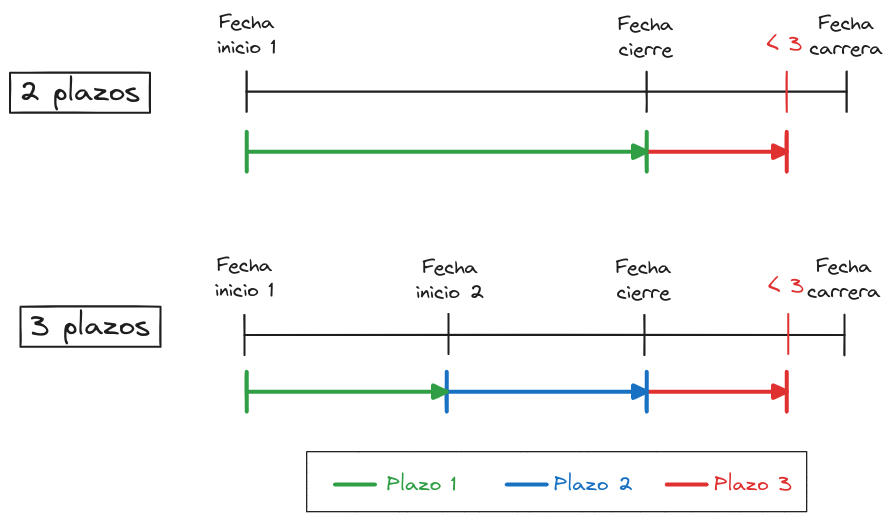
\includegraphics[width=\textwidth]{plazos.png}
			\captionof{figure}{Plazos de inscripción}
		\end{minipage}

		Como se puede observar en el anterior diagrama, en el caso de que haya solo dos plazos
		tanto la fecha de cierre como la fecha de inicio pertenecen al primer plazo. En el caso
		de que haya tres plazos, la fecha de inicio del segundo plazo y la fecha de cierre
		pertenecen al segundo plazo. En ambos casos, tres días antes del comienzo de la carrera
		es el día límite para inscribirse.
	\item \textbf{Edad}: se aplica AVL en el límite entre mayor y menor de edad, y en algunos
		límites de las categorías de edad para comprobar que todo funciona correctamente, es
		decir: \begin{itemize}
			\item Atleta menor de edad por un día en el día de la carrera
			\item Atleta con mayoría de edad cumplida el mismo día de la carrera
			\item Atleta con 35 años cumplidos el día de la carrera
		\end{itemize}
\end{itemize}
